\documentclass{article}

\usepackage{tikz}

\author{Yeoun Chan Kim \and John Strauser \and Xuanang Wang}

\title{CS440 Report}

\begin{document}

\maketitle

\section*{Part 1}

\begingroup
\centering

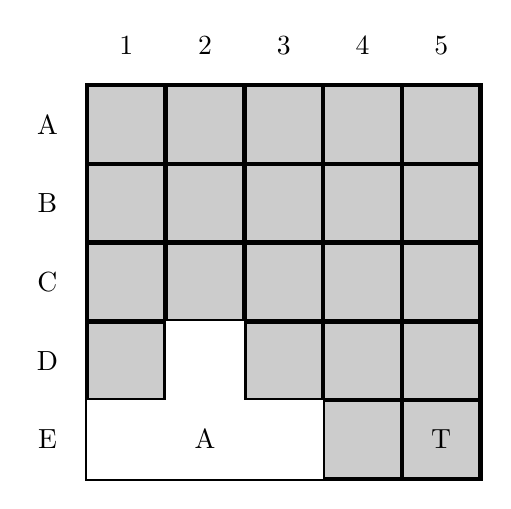
\begin{tikzpicture}
\draw [ultra thick, draw=black, fill=black!20!white] (0,0) grid  (5,5) rectangle (0,0);
\fill[white] (0,0) rectangle(1, 1);
\fill[white] (1,0) rectangle(2, 1); 
\fill[white] (2,0) rectangle(3, 1); 
\fill[white] (1,1) rectangle(2, 2); 
\node at (+1.5,+0.5) {A};
\node at (+4.5,+0.5) {T};
\node at (-0.5,+0.5) {E};
\node at (-0.5,+1.5) {D};
\node at (-0.5,+2.5) {C};
\node at (-0.5,+3.5) {B};
\node at (-0.5,+4.5) {A};
\node at (+0.5,+5.5) {1};
\node at (+1.5,+5.5) {2};
\node at (+2.5,+5.5) {3};
\node at (+3.5,+5.5) {4};
\node at (+4.5,+5.5) {5};
\end{tikzpicture}

\endgroup

\vspace{5mm} %5mm vertical space

a)Given the illustration above, Let (a, b) represent a unique state where a $\in$ \{ 1-5 \} and b $\in$ \{ A-E \}. We want to explain why the first move of the agent A in state (2, E) is to the east (3, E) rather than the north (2, D). Grey represents what agent cannot see and the white represents what agent can. According to the question, T in state (5, E) is the goal state. We calculate the Manhattan distance from A to T, which is 3 in the current situation: h(2, E) = 3. Let g(a, b)(c, d) represents the total distance cost from state (a, b) to state (c, d) in the A* searching path. Then in state (2, E), g(2, E)(2, E) = 0. Therefore, f(2, E) = 0 + 3 = 3. For all the state adjacent to (2, E) which are (1, E), (2, D), (3, E); the f value of each is (1, E): 4 + 1 = 5, (2, D): 4 + 1 = 5, (3, E): 2 + 1 = 3. According to the A* algorithm, we move the agent A to the position where the smallest f value holds. Therefore, the agent would move to the east (3, E) rather than the north(2, D) or (1, E).
\hspace{5mm}

b)Let S be the state in the finite gridworld, S{\small (s)} denotes the starting state, S{\small (c)} denotes the current state and S{\small (g)} denotes the goal state. For any S{\small (c)}, let h(S{\small (c)}) be the Manhattan distance from S{\small (c)} to S{\small (g)}, let g(S{\small (c)}) be the distance traveled from S{\small (s)} to S{\small (c)}, let S{\small (c')} be any adjacent state of S{\small (c)} and h(S{\small (c')}) g(S{\small (c')}) be the corresponding h and g value. According to the A* algorithm, for any state S{\small (c)}, as long as it's adjacent is not blocked which given value infinity, we calculate the f value using the formula f{\small (c')} = h(S{\small (c')}) + g(S{\small (c')}) and choose the one with the smallest f value. Because of the fact that for each iteration we always choose the {\tiny (min)}f{\small (c')} to be the next step for the path, as long as one of the possible path from S{\small (s)} to S{\small (g)} is not blocked, we would guarantee to reach the target. To make the explanation more clear, we consider the illustration below where black cells represent blocked.

\vspace{5mm} %5mm vertical space

\begingroup
\centering

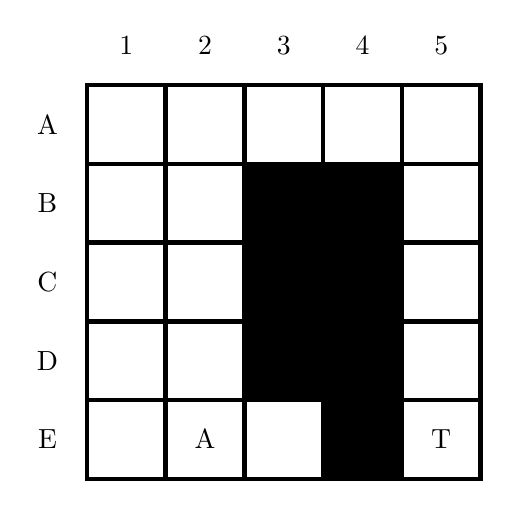
\begin{tikzpicture}
\draw [ultra thick, draw=black, fill=white] (0,0) grid  (5,5) rectangle (0,0);
\fill[black] (3,0) rectangle(4, 1);
\fill[black] (3,1) rectangle(4, 2); 
\fill[black] (3,2) rectangle(4, 3); 
\fill[black] (3,3) rectangle(4, 4); 
\fill[black] (2,1) rectangle(3, 2); 
\fill[black] (2,2) rectangle(3, 3); 
\fill[black] (2,3) rectangle(3, 4); 
\node at (+1.5,+0.5) {A};
\node at (+4.5,+0.5) {T};
\node at (-0.5,+0.5) {E};
\node at (-0.5,+1.5) {D};
\node at (-0.5,+2.5) {C};
\node at (-0.5,+3.5) {B};
\node at (-0.5,+4.5) {A};
\node at (+0.5,+5.5) {1};
\node at (+1.5,+5.5) {2};
\node at (+2.5,+5.5) {3};
\node at (+3.5,+5.5) {4};
\node at (+4.5,+5.5) {5};
\end{tikzpicture}

\endgroup

\vspace{5mm} %5mm vertical space

Because we are using the greedy approach, the next move of agent A at state (2, E) would be (3, E) (explained in part 1a)). However, when the state moves to (3, E), the dead-end situation occurred. Whenever we meet the situation like this, we would trace back to the parent cell of the dead ended cell, which is (2, E). After this, we would put (3, E) to closed list therefore the agent A would not able to go the (3, E) again even if f(3, E) is the smallest giving the situation the current state is (2, E).
\hspace{5mm}

However, if we put another block on (4, A), the agent would traverse from (2, E) vertically to (2, A); then go to (3, A) and backtrace to (2, A) because of the dead end.After that, the agent would go to (1, A) and vertically travel down to (1, E). In this situation, the open list is empty therefore the program returns false.

\section*{Part 2}
\hspace{5mm}
We run Repeated Forward A* break ties in favor of cells with smaller g-values for 30 times in 30 different 101 * 101 mazes. The expanded cell (runtime) for each is 
(10159, 10, 25194, 24938, 11969, 6033, 5226, 17104, 14849, 528, 1300, 341, 3424, 1623, 19212, 7388, 5365, 40, 1248, 2744, 4735, 15193, 1233, 1274, 6011, 1296, 977, 9868, 3322, 774).

Then we run Repeated Forward A* break ties in favor of cells with larger g-values for 30 times in 30 different 101 * 101 mazes. The expanded cell (runtime) for each is 
(2619, 8, 1739, 2167, 2967, 410, 1105, 1236, 2448, 110, 243, 151, 1327, 630, 3278, 623, 2014, 29, 414, 548, 1520, 1633, 289, 386, 1417, 294, 762, 1287, 679, 241).

The average for running RFA* in favor of smaller g-value 30 times is approximately 6605. And the average for running RFA* in favor of larger g-value 30 times is approximately 987 .

Through observation, we noticed that the run time of RFA* which break ties in favor of cells with smaller g-values has a significant amount of runtime increase compare to the one which break ties in favor of cells with larger g-values. The reason for that is, according to the Repeated A* algorithm, the only situation g-value would increase is when the agent break ties. This means the larger g-value is, the closer agent is to the target cell. Therefore, breaking ties in favor of cells with larger g-value is more efficient in terms of runtime.


\section*{Part 3}
\hspace{5mm}
As stated in part 2, the expanded cell (runtime) for RFA* in favor of cells with larger g-values is
(2619, 8, 1739, 2167, 2967, 410, 1105, 1236, 2448, 110, 243, 151, 1327, 630, 3278, 623, 2014, 29, 414, 548, 1520, 1633, 289, 386, 1417, 294, 762, 1287, 679, 241).

Then we run Repeated Backward A* in favor of cells with larger g-values for 30 times in the same 30 different 101 * 101 mazes. the expanded cell (runtime) for each is 
(7454, 6, 8924, 6978, 10492, 1755, 7668, 8889, 7977, 408, 648, 251, 4338, 1681, 16762, 6206, 5607, 25, 1321, 1447, 3738, 5504, 458, 929, 4814, 1579, 742, 7747, 1269, 266).

The average for running RFA* 30 times is approximately 987. And the average for running RBA* 30 times is approximately 4196.

Through observation, we notice that RFA* is way faster than RBA*.  

\section*{Part 4}
\hspace{5mm}
The h-value calculates the sum of the distances of the tiles from their goal positions. Since the agent cannot move along diagonals, the distance is the sum of the horizontal and vertical distances. The formula that we used in our project to calculate Manhattan distance is Manhattan Distance = abs(Horizontal Distance) + abs(Vertical Distance). This is only consistent when agent is allowed to move only in the four main compass directions. The counterexample is (Use diagram and explain if agent can move diagonally if goal position is three diagonal steps away, Manhattan distance is 6 so it becomes inconsistent).
From the lecture slides, the heuristic function is said to be consistent if
        for all(n, a, n’) : h(n) <= c(n, a, n’) + h(n’)
where c(n, a, n’) is the step cost for going from n to n’ using action a.
The adaptive A* leaves initially consistent h-values consistent because it changes consistent h-values into more informed consistent h-values. In states spaces, it can find the shortest path even if action cost can increase because consistent h-values remain consistent after action cost increases.

\section*{Part 5}
\hspace{5mm}
As stated in part 2, the expanded cell (runtime) for RFA* in favor of cells with larger g-values is
(2619, 8, 1739, 2167, 2967, 410, 1105, 1236, 2448, 110, 243, 151, 1327, 630, 3278, 623, 2014, 29, 414, 548, 1520, 1633, 289, 386, 1417, 294, 762, 1287, 679, 241).

Then we run Adaptive A* in favor of cells with larger g-values for 30 times in the same 30 different 101 * 101 mazes. the expanded cell (runtime) for each is
(2671, 8, 1846, 2109, 2958, 429, 1044, 1201, 2383, 212, 268, 149, 1338, 545, 3681, 637, 2079, 17, 413, 556, 1530, 1655, 281, 377, 1441, 297, 767, 1254, 657, 235).

The average for running RFA* 30 times is approximately 987. And the average for running Adaptive A* 30 times is approximately 1101.

Through observation, we notice that Adaptive A* is slower than RFA* in terms of runtime. This make sense because the calculation of h-value of Adaptive A* at iteration i is depended on its previous iteration (i-1). And we need to run RFA* on the (i-1)th iteration in order to get the so called 'old closed list' which being needed to calculate the h-value to run Adaptive A*. Also, we can notice that the runtime difference between Adaptive A* and RFA* is not very significant. This also make sense because after running the (i-1)th iteration using RFA*, the old closed list would have a very good information (g-value for each expanded node) which can navigate the agent to the target fast instead of searching for a path which costs more.

\section*{Part 6}
\hspace{5mm}
For further implementations, we can use breadth first search algorithm to reduce memory consumption. Since the tree-pointers can be implemented with two bits per cell, we can use little memory.  Rather than using multiple paths, we can do a local search at a current node. Since 1 byte = 8 bits, we can store 4 cells into 1 byte. If the gridworld is size of 1001 * 1001, it contains 1,002,001 cells. Divide 1,002,001 by 4 we get 250,500.25, which means we need 250,500.25 bytes. It is equivalent to 244.629 Kilobytes. If we can operate within memory limit of 4 Megabytes, 4 Megabytes is equivalent to 4194304 bytes. Since 4 cells can be stored in 1 byte, 4,194,304 * 4 = 16,777,216 cells. If we take the square root of 16,777,216, it is 4,096. It means we can operate 4,096 * 4,096 gridworld within memory limit of 4 Megabytes.



\end{document}